\section{Numerische Lösung nicht linearer Gleichungssysteme}

\begin{remark}
    LGS = lineares Gleichungssystem, NGS = nichtlineares Gleichungssystem
\end{remark}

\begin{example2}{Einleitendes Beispiel}

    \begin{minipage}{0.4\linewidth}
        Gesucht sind die Lösungen des Gleichungssystems:
    \end{minipage}
    \begin{minipage}{0.55\linewidth}
        \vspace{-6mm}
    $$f_1(x_1, x_2) = x_1^2 + x_2 - 11 = 0$$
    $$f_2(x_1, x_2) = x_1 + x_2^2 - 7 = 0$$
    \end{minipage}
    \vspace{1mm}\\
    Diese lassen sich interpretieren als die Nullstellen der Funktion:
    \vspace{-2mm}
    $$\textbf{f}: \R^2 \to \R^2 \quad \textbf{f}(x) = \begin{psmallmatrix} f_1 (x_1, x_2) \\ f_2 (x_1, x_2) \end{psmallmatrix} = \begin{psmallmatrix} x_1^2 + x_2 - 11 \\ x_1 + x_2^2 - 7 \end{psmallmatrix} = \begin{psmallmatrix} 0\\ 0 \end{psmallmatrix}$$
    Ein solches System lässt sich nicht in die Form $Ax = b$ bringen. 

    \begin{minipage}{0.59\linewidth}
    Geometrisch lassen sich die Lösungen als Schnittpunkte der beiden Funktionen interpretieren.\\
    Explizite Darstellung der Kurven:
    \vspace{-2mm}
    $$x_2 = 11 - x_1^2 \text{ und } x_2 = \sqrt{7 - x_1}$$
    Schnittpunkte:
    \vspace{-2mm}
    $$\overline{\textbf{x}_1} = \begin{psmallmatrix} 3 \\ 2 \end{psmallmatrix}, \quad \overline{\textbf{x}_2} = \begin{psmallmatrix} -2.8 \\ 3.2 \end{psmallmatrix}$$
    $$\overline{\textbf{x}_3} = \begin{psmallmatrix} -3.8 \\ -3.3 \end{psmallmatrix}, \quad \overline{\textbf{x}_4} = \begin{psmallmatrix} 3.4 \\ -1.7 \end{psmallmatrix}$$
    \end{minipage}
    \begin{minipage}{0.4\linewidth}
    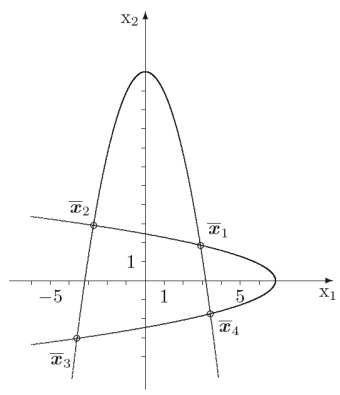
\includegraphics[width=\linewidth]{einleitendes_bsp_kap5.png}
    \end{minipage}
\end{example2}

\raggedcolumns

\subsection{Funktionen mit mehreren Variablen}

\begin{definition}{Skalarwertige Funktionen}
    $f: D \subset \R^n \to W \subset \R$
    \vspace{-2mm}
    $$(x_1, x_2, \ldots, x_n) \mapsto y = f(x_1, x_2, \ldots, x_n)$$
    Unter einer Funktion $f$ mit $n$ unabhängigen Variablen $x_1, \ldots, x_n$ und einer abhängigen Variablen $y$ versteht man eine Vorschrift, 
    die jedem geordneten Zahlentupel $(x_1, x_2, \ldots, x_n)$ aus einer Definitionsmenge $D \subset \R^n$ genau ein Element $y \in W \subset \R$ zuordnet.
    \vspace{2mm} \\
    Da das Ergebnis $y \in \R$ ein Skalar (eine Zahl) ist, redet man auch von einer \textbf{skalarwertigen Funktion}.
\end{definition}

\begin{concept}{Vektorwertige Funktion} gibt einen \textbf{Vektor} zurück (statt Skalar)\\
    Sei $\textbf{f}: \R^n \to \R^m$ eine Funktion mit $n$ Variablen.
    \vspace{-2mm}
    $$\textbf{f}(x_1 \ldots, x_n) = \begin{psmallmatrix} y_1 = f_1(x_1, x_2, \ldots, x_n) \\ y_2 = f_2(x_1, x_2, \ldots, x_n) \\ \vdots \\ y_m = f_m(x_1, x_2, \ldots, x_n) \end{psmallmatrix}$$
    wobei die $m$ Komponenten $f_i: \R^n \to \R$ für $i = 1, 2, \ldots, n$ von $\textbf{f}$ wieder \textbf{skalarwertige} Funktionen sind.
\end{concept}

\begin{corollary}{Eigenschaften von skalar- und vektorwertigen Funktionen}
    \begin{itemize}
        \item Skalar- und vektorwertige Funktionen mit mehreren Variablen werden auch \textbf{multivariat} genannt.
        \item Wie bei einem Vektor $\textbf{x}$ stellen wir zur besseren Unterscheidbarkeit vektorwertige Funktionen $\textbf{f}$ fett dar, im Gegensatz zu Skalaren $x$ und skalarwertigen Funktionen $f$.
        \item Wir werden uns bei der Lösung nichtlinearer Gleichungssysteme auf vektorwertige Funktionen $\textbf{f} = \R^n \to \R^n$ konzentrieren.
    \end{itemize}
\end{corollary}



\begin{example2}{Grundlegende Rechenoperationen} \\
    können als Skalarwertige Funktionen $f: \R^2 \to \R$ oder als \\
    Vektorwertige Funktionen $\textbf{f}: \R^2 \to \R^2$ interpretiert werden:
    $$f(x, y) = x + y, \quad g(x, y) = x \cdot y, \quad h(x, y) = x^2 + y^2$$
    $$\textbf{f}(x, y) = \begin{psmallmatrix} x + y \\ x \cdot y \end{psmallmatrix}, \quad \textbf{g}(x, y) = \begin{psmallmatrix} x \cdot y \\ x^2 + y^2 \end{psmallmatrix}$$
\end{example2}

\begin{example2}{Lineare Funktionen von LGS}
    Gebe die lineare Funktion $\textbf{f}: \R^3 \to \R^3$ an, für welche die Lösung $\textbf{x}$ des LGS:
    $$\textbf{Ax} = \textbf{b} \text{ mit } \textbf{A} = \begin{psmallmatrix} 4 & -1 & 1 \\ -2 & 5 & 1 \\ 1 & -2 & 5 \end{psmallmatrix} \text{ und } \textbf{b} = \begin{psmallmatrix} 1 \\ 2 \\ 3 \end{psmallmatrix} \text{ gerade } \textbf{f(x)} = \textbf{0} \text{ ergibt:}$$
    $$\textbf{A} \overrightarrow{\textbf{x}} = \overrightarrow{\textbf{b}} \Rightarrow \underbrace{\textbf{A} \overrightarrow{\textbf{x}} - \overrightarrow{\textbf{b}} = \overrightarrow{\textbf{0}}}_{\overrightarrow{\textbf{f}}(\overrightarrow{\textbf{x}})} \Rightarrow \overrightarrow{\textbf{f}}(x_1, x_2, x_3) = 0 \begin{psmallmatrix} x_1 \\ x_2 \\ x_3 \end{psmallmatrix} = \begin{psmallmatrix} 0 \\ 0 \\ 0 \end{psmallmatrix}$$
    \tcblower
    $$\overrightarrow{\textbf{f}}(\overrightarrow{\textbf{x}}) = \textbf{A} \overrightarrow{\textbf{x}} - \overrightarrow{\textbf{b}} = \begin{psmallmatrix} 4 & -1 & 1 \\ -2 & 5 & 1 \\ 1 & -2 & 5 \end{psmallmatrix} \begin{psmallmatrix} x_1 \\ x_2 \\ x_3 \end{psmallmatrix} - \begin{psmallmatrix} 5 \\ 11 \\ 12 \end{psmallmatrix}$$
    %Die Funktion $\textbf{f}$ ist gegeben durch: (\textcolor{pink}{\textbf{solved by copilot so no guarantees}})
    $$\textbf{f}(x_1, x_2, x_3) = \begin{psmallmatrix} f_1 = 4x_1 - x_2 + x_3 - 5 \\ f_2 = -2x_1 + 5x_2 + x_3 - 11 \\ f_3 = x_1 - 2x_2 + 5x_3 - 12 \end{psmallmatrix}$$
\end{example2}


\subsubsection{Darstellungsformen}

\begin{concept}{Analytische Darstellung}
    \begin{itemize}
        \item \textbf{Explizite Darstellung:} $y = f(x_1, \ldots, x_n)$
        \begin{itemize}
            \item die Funktionsgleichung ist nach einer Variablen aufgelöst
            \item Beispiel: $y = 2 \cdot e^(x_1^2 + x_2^2)$
        \end{itemize}
        \item \textbf{Implizite Darstellung:} $F(x, y) = 0$
        \begin{itemize}
            \item die Funktionsgleichung ist nicht nach einer Variablen aufgelöst
            \item daher handelt es sich um eine Funktion mit nur $n-1$ unabhängigen Variablen
            \item Beispiel: $x_1^2 + x_2^2 - 1 = 0$
        \end{itemize}
        \item \textbf{Parameterdarstellung:} $x = x(t), y = y(t)$
        \begin{itemize}
            \item die Funktion wird durch eine Kurve im Raum beschrieben
            \item Beispiel: $x(t) = \cos(t), y(t) = \sin(t)$
        \end{itemize}
    \end{itemize}
\end{concept}

\begin{concept}{Darstellung durch Wertetabelle}
    Sei $f: \R^n \to \R^m$ eine Funktion.\\
    In die vorausgesetzte Funktionsgleichung $z = f(x,y)$ werden die Werte der unabhängigen Variablen $x$ und $y$ eingesetzt (der Reihe nach).\\
    So erhält man eine Wertetabelle, bzw. Matrix:\\
    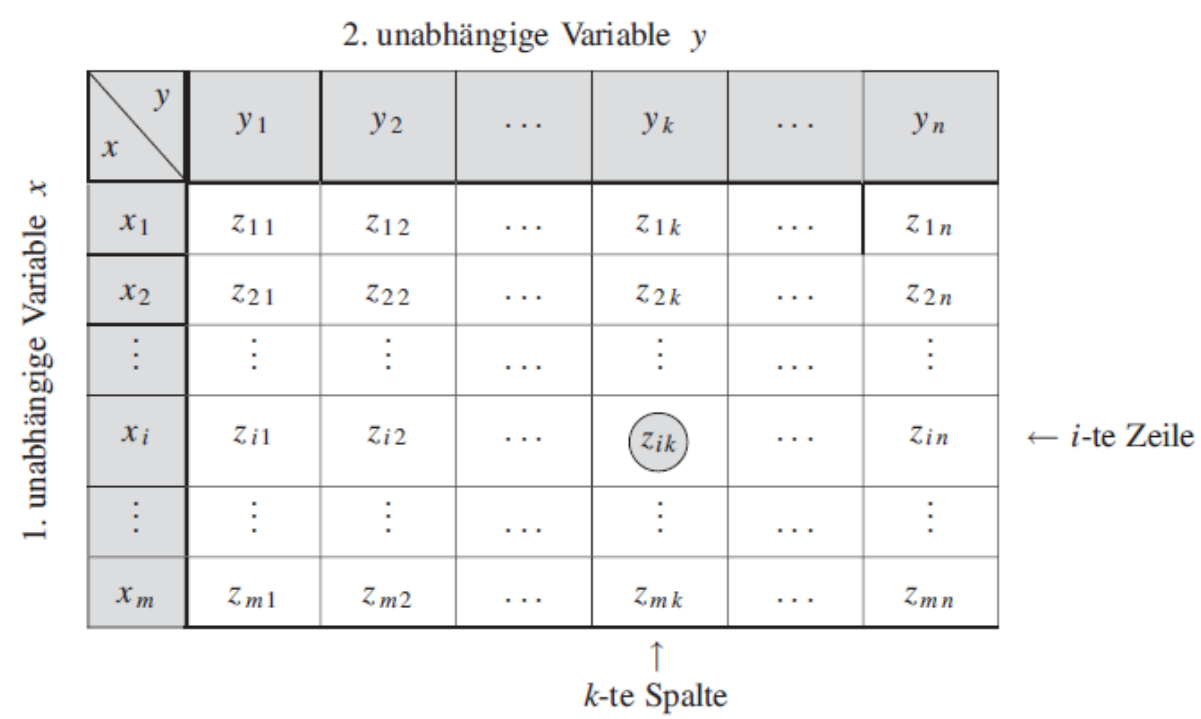
\includegraphics[width=0.9\linewidth]{wertetabelle_darstellung.png}
\end{concept}

\begin{concept}{Grafische Darstellung}
    Wir beschränken uns hier auf skalarwertige Funktionen mit zwei unabhängigen Variablen $f: \R^2 \to \R$.\\
    Dazu betrachten wir die Funktion $z = f(x, y)$ in einem dreidimensionalen kartesischen Koordinatensystem:
    
    \paragraph{Darstellung einer Funktion als Fläche im Raum}
    Die Funktion $f$ ordnet jedem Punkt $(x, y) \in D$ in der Ebene einen Wert $z=f(x, y)$ zu, der als Höhenkoordinate verstanden werden kann. 
    Durch die Anordnung der Punkte ( $x, y, f(x, y)$ ) im dreidimensionalen Koordinatensystem wird eine über dem Definitionsbereich $D$ liegende Fläche ausgezeichnet:

    \includegraphics[width=\linewidth]{funktion_als_fläche_im_raum.png}
    
    \paragraph{Schnittkurvendiagramm}
    Wird die Fläche $z=f(x, y)$ bei einer konstanten Höhe $z=$ const. geschnitten, ergibt sich eine Schnittkurve. 
    Wird diese in die $(x, y)$-Ebene projiziert, spricht man von einer Höhenlinie bzw. bei der Abbildung von einem Höhenliniendiagramm., wie wir es z.B. von Wanderkarten her kennen. 
    Natürlich kann man auch andere Schnitte als $z=$ const. (Schnittebene parallel zur $(x, y)$-Ebene) wählen, z.B. $x=$ const. (Schnittebene parallel zur $(y, z)$-Ebene) oder $y=$ const. (Schnittebene parallel zur $(x, z)$-Ebene):

    \begin{minipage}{0.6\linewidth}
    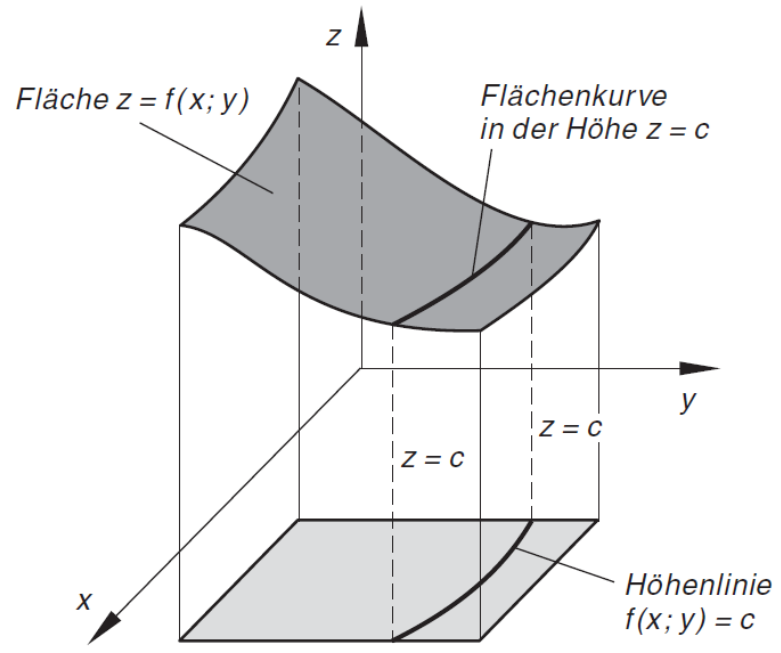
\includegraphics[width=\linewidth]{grafische_darstellung_detailed.png}
    \end{minipage}
    \begin{minipage}{0.38\linewidth}
    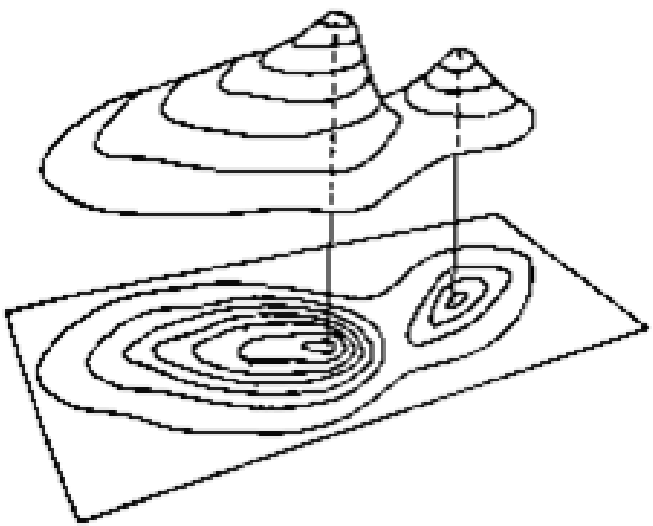
\includegraphics[width=\linewidth]{grafische_darstellung2.png}\\
    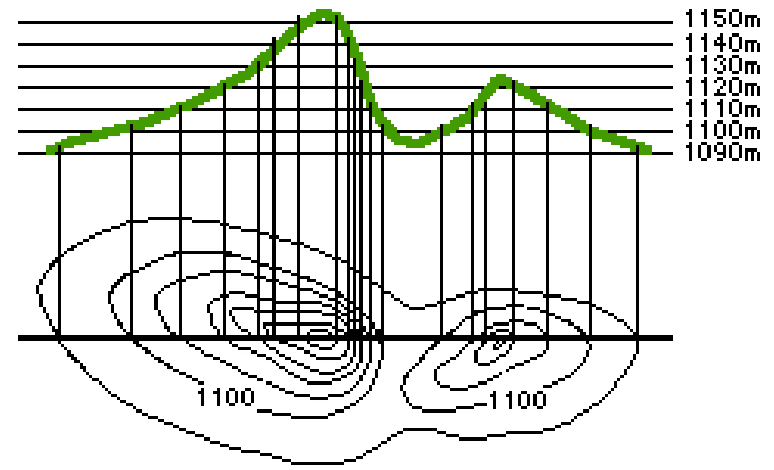
\includegraphics[width=\linewidth]{grafische_darstellung3.png}
    \end{minipage}
\end{concept}

\subsection{Partielle Ableitungen}

\begin{definition}{Partielle Ableitungen 1. Ordnung}\\
Unter den partiellen Ableitungen 1. Ordnung einer Funktion $z = f(x,y)$ an der Stelle $(x,y)$ werden die folgenden Grenzwerte verstanden:

\textbf{Partielle Ableitung nach x:}
$$\frac{\partial f}{\partial x}(x,y) = \lim_{\Delta x \rightarrow 0} \frac{f(x + \Delta x, y) - f(x,y)}{\Delta x}$$

\textbf{Partielle Ableitung nach y:}
$$\frac{\partial f}{\partial y}(x,y) = \lim_{\Delta y \rightarrow 0} \frac{f(x, y + \Delta y) - f(x,y)}{\Delta y}$$

Alternative Notationen: $f_x(x,y)$, $f_y(x,y)$ oder $f_x$, $f_y$
\end{definition}

\begin{theorem}{Partielle Ableitung}
In einer Dimension
$$
f^{\prime}\left(x_0\right)=\lim _{\Delta x \rightarrow 0} \frac{\left(f\left(x_0+\Delta x\right)-f\left(x_0\right)\right)}{\Delta x}
$$

\textcolor{frog}{\textbf{In mehreren Dimensionen}}
$$\text{1. Ableitung nach x: } f_x=\frac{\partial f}{\partial x}(x, y)=\lim _{\Delta x \rightarrow 0} \frac{f(x+\Delta x, y)-f(x, y)}{\Delta x}$$
$$\text{2. Ableitung nach y: } f_y=\frac{\partial f}{\partial y}(x, y)=\lim _{\Delta y \rightarrow 0} \frac{f(x, y+\Delta y)-f(x, y)}{\Delta y}$$
\end{theorem}



\begin{KR}{Partielle Ableitungen berechnen}
    \begin{enumerate}
        \item Variable identifizieren: Bestimme, nach welcher Variable abgeleitet werden soll
        \item Alle anderen Variablen werden während der Ableitung als Konstanten betrachtet
        \item Standardableitungsregeln anwenden und Ergebnis korrekt notieren
    \end{enumerate}
\end{KR}

\begin{example2}{Partielle Ableitungen berechnen}
Berechne die partiellen Ableitungen von $z = f(x,y) = 3xy^2 + \ln(x^3 y^2)$ an der Stelle $(x_0, y_0) = (-1, 1)$.
\paragraph{In beiden Dimensionen berechnen}
$$f_x = 3 \cdot 1 \cdot y^2 + \frac{1}{x^3 y^2} \cdot 3x^2 \cdot y^2 = 3y^2 + \frac{3}{x}$$
$$f_y = 3x \cdot 2y + \frac{1}{x^3 y^2} \cdot x^3 \cdot 2y = 6xy + \frac{2}{y}$$
An der Stelle $(-1, 1)$:\\
$f_x(-1, 1) = 3 \cdot 1^2 + \frac{3}{-1} = 3 - 3 = 0$\\
$f_y(-1, 1) = 6 \cdot (-1) \cdot 1 + \frac{2}{1} = -6 + 2 = -4$
\end{example2}

\begin{example2}{Tangentensteigung}
$z=f(x, y)=3 x y^3+10 x^2 y+5 y+3 y \cdot \sin (5 x y)$
$$\frac{\partial f}{\partial x}(x, y)=3 \cdot 1 \cdot y^3+10 \cdot 2 x \cdot y+0+3 y \cdot \cos (5 x y) \cdot 5 \cdot 1 \cdot y$$
$$\frac{\partial f}{\partial y}(x, y)=3 x \cdot 3 y^2+10 x^2 \cdot 1+5 \cdot 1+(3 \cdot 1 \cdot \sin (5 x y)+3 y \cdot \cos (5 x y) \cdot 5 x \cdot 1)$$

Steigung der beiden Tangenten in $x-$/$y$-Richtung im Punkt: \\
$\left(x_0, y_0\right)=(-1,1)$
\end{example2}

\subsection{Jacobi-Matrix und Linearisierung}

\begin{definition}{Jacobi-Matrix}\\
Sei $f: \mathbb{R}^n \rightarrow \mathbb{R}^m$ mit $y = f(x)$ und $x = (x_1, x_2, ..., x_n)^T \in \mathbb{R}^n$. 
Die Jacobi-Matrix enthält sämtliche partiellen Ableitungen 1. Ordnung von $f$ und ist definiert als:
$$f(x) = \begin{psmallmatrix}
    y_1=f_1(x) \\
    y_2=f_2(x) \\
    \vdots \\
    y_m=f_m(x)
\end{psmallmatrix} \rightarrow 
Df(x) := \begin{bsmallmatrix}
\frac{\partial f_1}{\partial x_1}(x) & \frac{\partial f_1}{\partial x_2}(x) & \cdots & \frac{\partial f_1}{\partial x_n}(x) \\
\frac{\partial f_2}{\partial x_1}(x) & \frac{\partial f_2}{\partial x_2}(x) & \cdots & \frac{\partial f_2}{\partial x_n}(x) \\
\vdots & \vdots & \ddots & \vdots \\
\frac{\partial f_m}{\partial x_1}(x) & \frac{\partial f_m}{\partial x_2}(x) & \cdots & \frac{\partial f_m}{\partial x_n}(x)
\end{bsmallmatrix}$$
\end{definition}

\begin{concept}{Linearisierung}
Die verallgemeinerte \textcolor{purple}{\textbf{Tangentengleichung}}
$$g(x) = f(x^{(0)}) + Df(x^{(0)}) \cdot (x - x^{(0)})$$
beschreibt eine lineare Funktion und es gilt $f(x) \approx g(x)$ in einer Umgebung eines gegebenen Vektors $x^{(0)}=(x_1^{(0)}, x_2^{(0)}, \ldots, x_n^{(0)})^T \in \mathbb{R}^n$. 
Man spricht von der \textbf{Linearisierung} der Funktion $y = f(x)$ in einer Umgebung von $x^{(0)}$ (ein hochgestellter Index in Klammern $x^{(k)}$ bezeichnet wie bisher einen Vektor aus $\R^n$ nach der $k$-ten Iteration).
\end{concept}

\begin{corollary}{Tangentialebene}
    Für den speziellen Fall $f: \mathbb{R}^2 \longrightarrow \mathbb{R}$ mit $y=f(x_1, x_2)$ und $\boldsymbol{x}^{(0)}=(x_1^{(0)}, x_2^{(0)})^T \in \mathbb{R}^2$ 
    ist die Jacobi-Matrix nur ein Zeilenvektor mit zwei Elementen, nämlich:
    $$Df(x^{(0)}) = \left(\frac{\partial f}{\partial x_1}(x_1^{(0)}, x_2^{(0)}), \frac{\partial f}{\partial x_2}(x_1^{(0)}, x_2^{(0)})\right)$$
    Dann liefert die Linearisierung $g(x_1, x_2)$:\\ 
    $$=f(x_1^{(0)}, x_2^{(0)}) + \left(\frac{\partial f}{\partial x_1}(x_1^{(0)}, x_2^{(0)}), \frac{\partial f}{\partial x_2}(x_1^{(0)}, x_2^{(0)})\right) \cdot \binom{x_1 - x_1^{(0)}}{x_2 - x_2^{(0)}}$$
    $$= f(x_1^{(0)}, x_2^{(0)}) + \frac{\partial f}{\partial x_1}(x_1^{(0)}, x_2^{(0)}) \cdot (x_1 - x_1^{(0)}) + \frac{\partial f}{\partial x_2}(x_1^{(0)}, x_2^{(0)}) \cdot (x_2 - x_2^{(0)})$$
    die Gleichung der Tangentialebene.

    Sie enthält sämtliche im Flächenpunkt 
    $\stackrel{\bullet}{P}=\left(x_1^{(0)}, x_2^{(0)}, f(x_1^{(0)}, x_2^{(0)})\right)$ \\
    an die Bildfläche von $y=f(x_1, x_2)$ angelegten Tangenten.
\end{corollary}

\begin{KR}{Jacobi-Matrix berechnen und linearisieren}\\
Sei $f: \mathbb{R}^n \rightarrow \mathbb{R}^m$ mit $y = f(x)$ und $x = (x_1, x_2, ..., x_n)^T \in \mathbb{R}^n$. 
\vspace{-2mm}\\
\begin{enumerate}
    \item Identifiziere die Komponentenfunktionen $f_1, f_2, ..., f_m$ und \\ Variablen $x_1, x_2, ..., x_n$.
    \item Berechne die partiellen Ableitungen $\frac{\partial f_i}{\partial x_j}$ \\ für $i = 1, ..., m$ und $j = 1, ..., n$.
    \item Stelle die Jacobi-Matrix $Df(x)$ auf, indem du die partiellen Ableitungen in Matrixform anordnest.
    \item Werte die Jacobi-Matrix an einem Entwicklungspunkt $x^{(0)}$ aus, indem du die Werte der Variablen in die Matrix einsetzt.
    \item Berechne die Linearisierung der Funktion $g(x)$ mit der Formel: \\ $g(x) = f(x^{(0)}) + Df(x^{(0)}) \cdot (x - x^{(0)})$
\end{enumerate}
\end{KR}

\begin{example2}{Jacobi-Matrix und Linearisierung}
Berechnen Sie die Jacobi-Matrix von $f(x_1, x_2) = \begin{psmallmatrix} 5x_1 x_2 \\ x_1^2 x_2^2 + x_1 + 2x_2 \end{psmallmatrix}$ an der Stelle $\begin{psmallmatrix} x_1 \\ x_2 \end{psmallmatrix} = \begin{psmallmatrix} 1 \\ 2 \end{psmallmatrix}$ und linearisieren Sie die Funktion dort.

\textbf{Schritt 1:} Partielle Ableitungen berechnen
$$\frac{\partial f_1}{\partial x_1} = 5x_2, \quad \frac{\partial f_1}{\partial x_2} = 5x_1$$
$$\frac{\partial f_2}{\partial x_1} = 2x_1 x_2^2 + 1, \quad \frac{\partial f_2}{\partial x_2} = 2x_1^2 x_2 + 2$$

\textbf{Schritt 2:} Jacobi-Matrix aufstellen
$$Df(x_1, x_2) = \begin{bsmallmatrix} 5x_2 & 5x_1 \\ 2x_1 x_2^2 + 1 & 2x_1^2 x_2 + 2 \end{bsmallmatrix}$$

\textbf{Schritt 3:} An der Stelle $(1, 2)$ auswerten
$Df(1, 2) = \begin{bsmallmatrix} 10 & 5 \\ 9 & 6 \end{bsmallmatrix}$

\textbf{Schritt 4:} Funktionswert berechnen
$f(1, 2) = \begin{psmallmatrix} 10 \\ 9 \end{psmallmatrix}$

\textbf{Schritt 5:} Linearisierung
$g(x) = \begin{psmallmatrix} 10 \\ 9 \end{psmallmatrix} + \begin{bsmallmatrix} 10 & 5 \\ 9 & 6 \end{bsmallmatrix} \begin{psmallmatrix} x_1 - 1 \\ x_2 - 2 \end{psmallmatrix}$
\end{example2}



\begin{example2}{Linearisierung einer vektorwertigen Funktion}\\
    Linearisiere Sie für $x^{(0)}=(\pi / 4,0, \pi)^T$ der Funktion $f\left(x_1, x_2, x_3\right)$
    \vspace{2mm} \\
    \textbf{1. Jacobi-Matrix} $Df(x_1, x_2, x_3)$ bilden:
    $$f(x_1, x_2, x_3)=\begin{psmallmatrix} \sin (x_2+2 x_3) \\ \cos (2 x_1+x_2) \end{psmallmatrix}$$
    $$Df(x_1, x_2, x_3)= \begin{bmatrix} 0 & \cos (x_2+2 x_3) & 2 \cos (x_2+2 x_3) \\ -2 \sin (2 x_1+x_2) & -\sin (2 x_1+x_2) & 0 \end{bmatrix}$$
    \textbf{2. Startvektor} $x^{(0)}$ in Vektorwertige Funktion $f(x)$ und \\ Jacobi-Matrix $Df(x)$ \textbf{einsetzen:}
    $$f(\pi / 4,0, \pi)=f(x^{(0)})=\begin{psmallmatrix} \sin (0+2 \pi) \\ \cos (2 \cdot \pi / 4+0) \end{psmallmatrix}$$
    $$=\begin{psmallmatrix} 0 \\ 0 \end{psmallmatrix}, Df(x^{(0)})=\begin{bsmallmatrix} 0 & 1 & 2 \\ -2 & -1 & 0 \end{bsmallmatrix}$$
    \textbf{3. Verallgemeinerte Tangentengleichung:}
    $$g(x)=\underbrace{\begin{psmallmatrix} 0 \\ 0 \end{psmallmatrix}}_{f(x_0)}+\underbrace{\begin{bsmallmatrix} 0 & 1 & 2 \\ -2 & -1 & 0 \end{bsmallmatrix}}_{Df(x_0)} \cdot \underbrace{\begin{psmallmatrix} x_1-\pi / 4 \\ x_2-0 \\ x_3-\pi \end{psmallmatrix}}_{x-x_0}=\begin{psmallmatrix} x_2 + 2 x_3 - 2 \pi \\ -2 x_1 - x_2 + \pi / 2 \end{psmallmatrix}$$

\end{example2}

\raggedcolumns
\columnbreak

\subsection{Nullstellenbestimmung für NGS}

\begin{remark}
    Es gibt keine einfachen Methoden, um festzustellen, ob ein nichtlineares Gleichungssystem lösbar ist und wie viele Lösungen es hat. Deshalb entscheidet die Wahl
    einer «geeigneten Startnäherug» meist über erfolgt oder Misserfolg der eingesetzten numerischen Verfahren.
\end{remark}

\begin{definition}{Problemstellung zur Nullstellenbestimmung}\\
Gegeben sei $n \in \mathbb{N}$ und eine Funktion $f: \mathbb{R}^n \rightarrow \mathbb{R}^n$. Gesucht ist ein Vektor $\bar{x} \in \mathbb{R}^n$ mit $f(\bar{x}) = 0$.

Komponentenweise bedeutet dies: Gegeben sind $n$ Funktionen $f_i: \mathbb{R}^n \rightarrow \mathbb{R}$, die die Komponenten von $f$ bilden. Gesucht ist ein Vektor $\bar{x} \in \mathbb{R}^n$ mit $f_i(\bar{x}) = 0$ für $i = 1, ..., n$.
\end{definition}

\begin{concept}{Quadratisch konvergentes Newton-Verfahren} \small{(Quadratische Konv.)}\\
    \normalsize
    Gesucht sind Nullstellen von $f: \mathbb{R}^n \rightarrow \mathbb{R}^n$. Sei $x^{(0)}$ ein Startvektor in der Nähe einer Nullstelle. 
    Das Newton-Verfahren zur näherungsweisen Bestimmung dieser Nullstelle lautet:

    Lösung von $f(x)=0$ mit $f: \mathbb{R}^n \rightarrow \mathbb{R}^n$ für $n=0,1,2, \ldots$
    \begin{enumerate}
        \item Berechne $f(x^{(n)})$ und $D f(x^{(n)})$
        \item Berechne $\delta^{(n)}$ als Lösung des linearen Gleichungssystems
        $$Df(x^{(n)}) \cdot \delta^{(n)} = -f(x^{(n)})$$
        \item Setze $x^{(n+1)} := x^{(n)} + \delta^{(n)}$
    \end{enumerate}
\end{concept}

\begin{theorem}{Vereinfachtes Newton-Verfahren} (Lineare Konvergenz)

    Lösung von $f(x)=0$ mit $f: \mathbb{R}^n \rightarrow \mathbb{R}^n$ für $n=0,1,2, \ldots$
    \begin{enumerate}
        \item Berechne $f(x^{(n)})$ und $D f(x^{(0)})$
        \item Berechne $\delta^{(n)}$ als Lösung des lin. GS $D f\left(x^{(0)}\right) \cdot \delta^{(n)}=-f\left(x^{(n)}\right)$
        \item Setze $x^{(n+1)}:=x^{(n)}+\delta^{(n)}$
    \end{enumerate}
\end{theorem}

\begin{KR}{Newton-Verfahren für nichtlineare Gleichungssysteme}
\paragraph{Schritt 1: Funktionen und Jacobi-Matrix aufstellen}
Definiere $f(x) = 0$ und berechne die Jacobi-Matrix $Df(x)$.

\paragraph{Schritt 2: Startvektor wählen}
Wähle einen geeigneten Startvektor $x^{(0)}$ nahe der vermuteten Lösung.

\paragraph{Schritt 3: Iterative Berechnung}
Für jede Iteration $k$:
\begin{itemize}
    \item \textbf{Linearisierung um} $x^{(k)}$: Berechne $f(x^{(k)})$ und $Df(x^{(k)})$
    \item \textbf{Nullstelle der Linearisierung berechnen}: \\ Löse das LGS: $Df(x^{(k)}) \delta^{(k)} = -f(x^{(k)})$
    \item \textbf{Nächste Iteration}: Setze $x^{(k+1)} = x^{(k)} + \delta^{(k)}$
\end{itemize}
\vspace{2mm}
\textbf{Formel:}
        $x^{(k+1)}=x^{(k)}-(D f(x^{(k)}))^{-1} \cdot f(x^{(k)})$
\paragraph{Schritt 4: Konvergenzprüfung}
Prüfe Abbruchkriterien wie $$\|f(x^{(k+1)})\|_2 < \text{TOL} \text{ oder } \|x^{(k+1)} - x^{(k)}\|_2 < \text{TOL}$$

\paragraph{Schritt 5: Lösung interpretieren}
Die konvergierte Lösung $x^{(k)}$ ist eine Näherung für die Nullstelle.
\end{KR}

\begin{example2}{Newton-Verfahren anwenden} Löse das Gleichungssystem 
$$f(x_1, x_2) = \begin{psmallmatrix} 20 - 18x_1 - 2x_2^2 \\ -4x_2(x_1 - x_2^2) \end{psmallmatrix} = \begin{psmallmatrix} 0 \\ 0 \end{psmallmatrix}$$
mit dem Newton-Verfahren für den Startvektor $x^{(0)} = (1.1, 0.9)^T$.
\vspace{2mm}\\
\textbf{Schritt 1:} Jacobi-Matrix berechnen
$$Df(x_1, x_2) = \begin{bsmallmatrix} -18 & -4x_2 \\ -4x_2 & -4(x_1 - 3x_2^2) \end{bsmallmatrix}$$

\textbf{Schritt 2:} Erste Iteration ($k = 0$)
$$f(1.1, 0.9) = \begin{psmallmatrix} -1.42 \\ -0.036 \end{psmallmatrix}$$
$$Df(1.1, 0.9) = \begin{bsmallmatrix} -18 & -3.6 \\ -3.6 & -5.32 \end{bsmallmatrix}$$

LGS lösen: $\begin{bsmallmatrix} -18 & -3.6 \\ -3.6 & -5.32 \end{bsmallmatrix} \delta^{(0)} = \begin{psmallmatrix} 1.42 \\ 0.036 \end{psmallmatrix}$
$\Rightarrow \delta^{(0)} = \begin{psmallmatrix} -0.0822 \\ 0.0178 \end{psmallmatrix}$
$$x^{(1)} = \begin{psmallmatrix} 1.1 \\ 0.9 \end{psmallmatrix} + \begin{psmallmatrix} -0.0822 \\ 0.0178 \end{psmallmatrix} = \begin{psmallmatrix} 1.0178 \\ 0.9178 \end{psmallmatrix}$$

Weitere Iterationen führen zur Konvergenz.
\end{example2}

\begin{example2}{Beispiel mit Newton-Verfahren}
    
Gegeben sind zwei Gleichungen und der Start-Vektor $x^{(0)}=(2,-1)^T$

$$
1-x^2=y^2, \quad \frac{(x-2)^2}{a}+\frac{(y-1)^2}{b}=1
$$


Umwandlung in Funktionen $f_1, f_2=0$

$$
f_1(x, y)=1-x^2-y^2=0, \quad f_2(x, y)=\frac{(x-2)^2}{a}+\frac{(y-1)^2}{b}-1=0
$$


Vektorwertige Funktion und Jacobi-Matrix bilden

$$
D f(x, y)=\left(\begin{array}{cc}
-2 x & -2 y \\
\frac{2 x-4}{a} & \frac{2 y-2}{b}
\end{array}\right), \quad f(x, y)=\binom{1-x^2-y^2}{\frac{(x-2)^2}{a}+\frac{(y-1)^2}{b}-1}
$$


Start-Vektor $x^{(0)}$ einsetzen

$$
D f(2,-1)=\left(\begin{array}{cc}
-4 & 2 \\
0 & -4 / b
\end{array}\right), \quad f(2,-1)=\binom{-4}{4 / b-1}
$$


Berechne $\delta^{(0)}$

$$
\left(D f\left(x^{(0)}\right) \mid-f\left(x^{(0)}\right)\right)=\left(\begin{array}{cc|c}
-4 & 2 & 4 \\
0 & -4 / b & -4 / b+1
\end{array}\right) \rightarrow \underbrace{\binom{-1}{0}}_{\delta^{(0)}}
$$


Berechne $x^{(1)}$

$$
x^{(1)}=\underbrace{\binom{2}{-1}}_{x^{(0)}}+\underbrace{\binom{-1}{0}}_{\delta^{(0)}}=\binom{1}{-1}
$$
\end{example2}

\subsection{Gedämpftes Newton-Verfahren}

\begin{corollary}{Gedämpftes Newton-Verfahren}

Nur in der Nähe der Nullstelle ist Konvergenz des Verfahrens garantiert!
\begin{enumerate}
    \item Berechne $f\left(x^{(n)}\right)$ und $D f\left(x^{(n)}\right)$
    \item Berechne $\delta^{(n)}$ als Lösung des lin. GS $D f\left(x^{(n)}\right) \cdot \delta^{(n)}=-f\left(x^{(n)}\right)$
    \item Finde das minimale $k \in\left\{0,1, \ldots, k_{\max }\right\}$ mit:
\end{enumerate}
$$
\left\|f\left(x^{(n)}+\frac{\delta^{(n)}}{2^k}\right)\right\|_2<\left\|f\left(x^{(n)}\right)\right\|_2
$$
Kein minimales $k$ gefunden $\rightarrow k=0$

4. Setze
$$
x^{(n+1)}:=x^{(n)}+\frac{\delta^{(n)}}{2^k}
$$
\end{corollary}

\begin{concept}{Dämpfung für bessere Konvergenz}\\
Falls die Jacobi-Matrix $Df(x^{(n)})$ schlecht konditioniert ist, kann das Standard Newton-Verfahren divergieren. Das gedämpfte Newton-Verfahren verwendet eine variable Schrittweite:

$$x^{(n+1)} = x^{(n)} + \frac{\delta^{(n)}}{2^p}$$

wobei $p$ das kleinste Element aus $\{0, 1, ..., p_{\max}\}$ ist, für das gilt:
$$\|f(x^{(n)} + \frac{\delta^{(n)}}{2^p})\|_2 < \|f(x^{(n)})\|_2$$
\end{concept}

\begin{KR}{Gedämpftes Newton-Verfahren}
\paragraph{Schritt 1-3: Wie beim Standard Newton-Verfahren}
Berechne $\delta^{(k)}$ durch Lösen von $Df(x^{(k)}) \delta^{(k)} = -f(x^{(k)})$.

\paragraph{Schritt 4: Dämpfungsparameter bestimmen}
Finde das kleinste $p \in \{0, 1, ..., p_{\max}\}$ mit:
$$\|f(x^{(k)} + \frac{\delta^{(k)}}{2^p})\|_2 < \|f(x^{(k)})\|_2$$

\paragraph{Schritt 5: Gedämpften Schritt ausführen}
Setze $x^{(k+1)} = x^{(k)} + \frac{\delta^{(k)}}{2^p}$.

\paragraph{Schritt 6: Bei Nicht-Konvergenz}
Falls kein geeignetes $p$ gefunden wird, setze $p = 0$ und fahre fort.
\end{KR}

\begin{example2}{Anwendung des gedämpften Newton-Verfahrens}\\
\textbf{Aufgabe:} Lösen Sie das System aus dem vorigen Beispiel mit gedämpftem Newton-Verfahren und einem 'schlechteren' Startvektor $x^{(0)} = (2, 2)^T$.
\vspace{1mm}\\
\textbf{Lösung:}
Das gedämpfte Newton-Verfahren konvergiert auch für diesen weiter entfernten Startvektor, während das ungedämpfte Verfahren divergieren würde. Die Dämpfung sorgt dafür, dass in jeder Iteration das Fehlerfunktional $\|f(x)\|_2$ abnimmt, wodurch die Stabilität erhöht wird.
\end{example2}

\begin{remark}
Das gedämpfte Newton-Verfahren ist besonders nützlich bei:
\begin{itemize}
    \item Schlecht konditionierten Problemen
    \item Startvektoren, die weit von der Lösung entfernt sind  
    \item Systemen mit mehreren Lösungen
    \item Praktischen Anwendungen, wo Robustheit wichtiger als Geschwindigkeit ist
\end{itemize}
\end{remark}

\raggedcolumns

\subsection{Anwendungsbeispiele}

\begin{example2}{LORAN-Navigationssystem}\\
\textbf{Aufgabe:} Bestimmen Sie die Position eines Empfängers aus den hyperbelförmigen Ortskurven:
$$f_1(x,y) = \frac{x^2}{186^2} - \frac{y^2}{300^2 - 186^2} - 1 = 0$$
$$f_2(x,y) = \frac{(y-500)^2}{279^2} - \frac{(x-300)^2}{500^2 - 279^2} - 1 = 0$$
\tcblower
\textbf{Lösung:}
\begin{enumerate}
    \item \textbf{Grafische Analyse:} Plotte beide Hyperbeln und bestimme visuell die vier Schnittpunkte
    \item \textbf{Numerische Lösung:} Verwende die geschätzten Positionen als Startvektoren für das Newton-Verfahren
    \item \textbf{Iteration:} Führe Newton-Verfahren mit Genauigkeit $\|f(x^{(k)})\|_2 < 10^{-5}$ durch
\end{enumerate}

Die vier Lösungen entsprechen den möglichen Positionen des Empfängers, wobei durch zusätzliche Information (z.B. dritter Sender) die eindeutige Position bestimmt werden kann.
\end{example2}

\begin{example2}{Dreidimensionales nichtlineares System}\\
\textbf{Aufgabe:} Lösen Sie das System:
$$f(x_1, x_2, x_3) = \begin{psmallmatrix}
x_1 + x_2^2 - x_3^2 - 13 \\
\ln\frac{x_2}{4} + e^{0.5x_3-1} - 1 \\
(x_2 - 3)^2 - x_3^3 + 7
\end{psmallmatrix} = \begin{psmallmatrix} 0 \\ 0 \\ 0 \end{psmallmatrix}$$

mit Startvektor $x^{(0)} = (1.5, 3, 2.5)^T$.
\tcblower
\textbf{Lösung:}
Dieses System erfordert das gedämpfte Newton-Verfahren aufgrund der komplexen nichtlinearen Terme. Die Jacobi-Matrix enthält sowohl polynomiale als auch transzendente Funktionen, was eine sorgfältige numerische Behandlung erfordert.
\end{example2}

\begin{example2}{Prüfungsaufgabe 5.1 - Newton-Verfahren}\\
\textbf{Aufgabe:} Gegeben ist das nichtlineare Gleichungssystem:
$$f(x_1, x_2) = \begin{psmallmatrix} x_1^2 + x_2^2 - 5 \\ x_1 x_2 - 2 \end{psmallmatrix} = \begin{psmallmatrix} 0 \\ 0 \end{psmallmatrix}$$

a) Berechnen Sie die Jacobi-Matrix $Df(x_1, x_2)$
b) Führen Sie zwei Schritte des Newton-Verfahrens mit Startvektor $x^{(0)} = (2, 1)^T$ durch
c) Geben Sie $\|f(x^{(2)})\|_2$ und $\|x^{(2)} - x^{(1)}\|_2$ an
\tcblower
\textbf{a) Jacobi-Matrix berechnen:}
$$f_1(x_1, x_2) = x_1^2 + x_2^2 - 5 \Rightarrow \frac{\partial f_1}{\partial x_1} = 2x_1, \frac{\partial f_1}{\partial x_2} = 2x_2$$
$$f_2(x_1, x_2) = x_1 x_2 - 2 \Rightarrow \frac{\partial f_2}{\partial x_1} = x_2, \frac{\partial f_2}{\partial x_2} = x_1$$

$$Df(x_1, x_2) = \begin{bsmallmatrix} 2x_1 & 2x_2 \\ x_2 & x_1 \end{bsmallmatrix}$$

\textbf{b) Newton-Verfahren:}

\textbf{Iteration 0 $\rightarrow$ 1:}
$$x^{(0)} = \begin{psmallmatrix} 2 \\ 1 \end{psmallmatrix} \Rightarrow
f(x^{(0)}) = \begin{psmallmatrix} 4 + 1 - 5 \\ 2 \cdot 1 - 2 \end{psmallmatrix} = \begin{psmallmatrix} 0 \\ 0 \end{psmallmatrix}$$

$\Rightarrow x^{(0)}$ ist bereits eine exakte Lösung! Aber rechnen wir weiter für die Demonstration:

Eigentlich sollten wir einen anderen Startpunkt wählen. \\ Nehmen wir $x^{(0)} = (2.2, 0.9)^T$:

$$f(2.2, 0.9) = \begin{psmallmatrix} 4.84 + 0.81 - 5 \\ 1.98 - 2 \end{psmallmatrix} = \begin{psmallmatrix} 0.65 \\ -0.02 \end{psmallmatrix}$$

$$Df(2.2, 0.9) = \begin{bsmallmatrix} 4.4 & 1.8 \\ 0.9 & 2.2 \end{bsmallmatrix}$$

LGS lösen: $Df(x^{(0)}) \delta^{(0)} = -f(x^{(0)})$

$\begin{bsmallmatrix} 4.4 & 1.8 \\ 0.9 & 2.2 \end{bsmallmatrix} \delta^{(0)} = \begin{psmallmatrix} -0.65 \\ 0.02 \end{psmallmatrix} \Rightarrow $
Lösung: $\delta^{(0)} = \begin{psmallmatrix} -0.1538 \\ 0.0769 \end{psmallmatrix}$

$$x^{(1)} = x^{(0)} + \delta^{(0)} = \begin{psmallmatrix} 2.2 \\ 0.9 \end{psmallmatrix} + \begin{psmallmatrix} -0.1538 \\ 0.0769 \end{psmallmatrix} = \begin{psmallmatrix} 2.0462 \\ 0.9769 \end{psmallmatrix}$$

\textbf{Iteration 1 $\rightarrow$ 2:}
$$f(2.0462, 0.9769) = \begin{psmallmatrix} 0.0415 \\ -0.0002 \end{psmallmatrix}$$

$$Df(2.0462, 0.9769) = \begin{bsmallmatrix} 4.0924 & 1.9538 \\ 0.9769 & 2.0462 \end{bsmallmatrix}$$

Nach Lösung des LGS: $\delta^{(1)} = \begin{psmallmatrix} -0.0103 \\ 0.0052 \end{psmallmatrix} \Rightarrow $
$x^{(2)} = \begin{psmallmatrix} 2.0359 \\ 0.9821 \end{psmallmatrix}$

\textbf{c) Fehlernormen:}
$$\|f(x^{(2)})\|_2 = \|f(2.0359, 0.9821)\|_2 = \|\begin{psmallmatrix} 0.0011 \\ 0.0000 \end{psmallmatrix}\|_2 = 0.0011$$

$$\|x^{(2)} - x^{(1)}\|_2 = \|\begin{psmallmatrix} -0.0103 \\ 0.0052 \end{psmallmatrix}\|_2 = 0.0115$$

\textbf{Interpretation:} Das Newton-Verfahren konvergiert quadratisch gegen die Lösung $(2, 1)^T$.
\end{example2}

\begin{example2}{Prüfungsaufgabe 5.2 - Jacobi-Matrix und Linearisierung}\\
\textbf{Aufgabe:} Gegeben ist die Funktion:
$$f(x, y, z) = \begin{psmallmatrix} e^{xy} + z^2 - 3 \\ \sin(x + y) - z \\ x^2 + y^2 + z^2 - 6 \end{psmallmatrix}$$

a) Berechnen Sie die Jacobi-Matrix $Df(x, y, z)$
b) Linearisieren Sie $f$ an der Stelle $(1, 0, 1)^T$
c) Welche geometrische Bedeutung hat die Linearisierung?
\tcblower
\textbf{a) Jacobi-Matrix:}
$$\frac{\partial f_1}{\partial x} = ye^{xy}, \quad \frac{\partial f_1}{\partial y} = xe^{xy}, \quad \frac{\partial f_1}{\partial z} = 2z$$
$$\frac{\partial f_2}{\partial x} = \cos(x + y), \quad \frac{\partial f_2}{\partial y} = \cos(x + y), \quad \frac{\partial f_2}{\partial z} = -1$$
$$\frac{\partial f_3}{\partial x} = 2x, \quad \frac{\partial f_3}{\partial y} = 2y, \quad \frac{\partial f_3}{\partial z} = 2z$$

$$Df(x, y, z) = \begin{bsmallmatrix} ye^{xy} & xe^{xy} & 2z \\ \cos(x + y) & \cos(x + y) & -1 \\ 2x & 2y & 2z \end{bsmallmatrix}$$

\textbf{b) Linearisierung an $(1, 0, 1)^T$:}
$$f(1, 0, 1) = \begin{psmallmatrix} e^0 + 1 - 3 \\ \sin(1) - 1 \\ 1 + 0 + 1 - 6 \end{psmallmatrix} = \begin{psmallmatrix} -1 \\ \sin(1) - 1 \\ -4 \end{psmallmatrix}$$

$$Df(1, 0, 1) = \begin{bsmallmatrix} 0 & 1 & 2 \\ \cos(1) & \cos(1) & -1 \\ 2 & 0 & 2 \end{bsmallmatrix}$$

Linearisierung: $g(x, y, z) = f(1, 0, 1) + Df(1, 0, 1) \cdot \begin{psmallmatrix} x - 1 \\ y - 0 \\ z - 1 \end{psmallmatrix}$

$$g(x, y, z) = \begin{psmallmatrix} -1 \\ \sin(1) - 1 \\ -4 \end{psmallmatrix} + \begin{bsmallmatrix} 0 & 1 & 2 \\ \cos(1) & \cos(1) & -1 \\ 2 & 0 & 2 \end{bsmallmatrix} \begin{psmallmatrix} x - 1 \\ y \\ z - 1 \end{psmallmatrix}$$

$$= \begin{psmallmatrix} -1 + y + 2(z-1) \\ \sin(1) - 1 + \cos(1)(x-1) + \cos(1)y - (z-1) \\ -4 + 2(x-1) + 2(z-1) \end{psmallmatrix}$$

\textbf{c) Geometrische Bedeutung:}
Die Linearisierung approximiert die nichtlineare Funktion $f$ in der Nähe des Punktes $(1, 0, 1)^T$ durch eine lineare Funktion. Dies entspricht der Tangentialebene an die durch $f = 0$ definierte Fläche im dreidimensionalen Raum.
\end{example2}



